\section{Appendix - Complete Schematics}
\includepdf[angle=90]{base-station}
\label{apx:base-station-sch}
\includepdf[angle=90]{power-board}
\label{apx:power-board-sch}
\includepdf[angle=90]{control-module}
\label{apx:control-module-sch}

\section{Appendix - Copyright Notices}
\emph{During the creation of this document, we avoided using any copyrighted works.}

% BEGIN BIBLIOGRAPHY
\thispagestyle{empty}
\pagestyle{empty}

\section{Appendix - References}

% Actual References
\renewcommand{\refname}{\centerline{\Large\bf References Cited}}
\bibliographystyle{simple}

\renewcommand{\refname}{}
\begin{thebibliography}{9}
\bibitem{link1} X10 Website \url{www.x10.com}
\bibitem{link2} Fuse Calculated \url{http://www.engbedded.com/fusecalc/}
\bibitem{link3} TFT 2.8" LCD \url{https://www.adafruit.com/products/1770}
\bibitem{link4} 5V Battery Backup \url{http://www.instructables.com/id/Simple-5v-battery-backup-circuit/}
\bibitem{link5} 12V Battery Backup \url{http://electronics.stackexchange.com/questions/96632/12v-battery-backup-supply-for-gprs-tracker}
\bibitem{link6} Capacitor Tut \url{http://www.electronics-tutorials.ws/capacitor/cap_2.html}
\bibitem{link7} Diode Ref Sheet \url{http://www.diodes.com/datasheets/ds28002.pdf}
\bibitem{link8} Solid State Relay \url{http://electronicdesign.com/components/electromechanical-relays-versus-solid-state-each-has-its-place}
\bibitem{link9} LDO Dropout \url{http://focus.ti.com/download/trng/docs/seminar/Topic\%209\%20-\%20Understanding\%20LDO\%20dropout.pdf}
\bibitem{link10} ISOCompare \url{http://www.tortech.com.au/isocompare}
\bibitem{link11} OSH Park \url{https://oshpark.com/pricing}
\bibitem{link12} 4PCB Service \url{http://www.4pcb.com/33-each-pcbs/}
\bibitem{link13} Sparkfun\url{http://sparkfun.com}
\bibitem{link14} Circuit Tutorial \url{http://www.allaboutcircuits.com/vol_5/chpt_2/2.html}
\bibitem{link15} Electrical \url{http://homerenovations.about.com/od/electrical/a/artelecbox.htm}
\bibitem{link16} GFI Outlet \url{http://diy.stackexchange.com/questions/15684/what-is-a-gfi-outlet-used-for-and-where-should-i-install-them}
\bibitem{link17} EAGLE Cad\url{http://www.cadsoftusa.com/download-eagle/freeware/}
\bibitem{link18} FreeRouter KiCad\url{http://www.freerouting.net/}
\bibitem{link19} Nest Website \url{http://nest.com}
\bibitem{link20} Forbes Article Nest Acquisition \url{http://www.forbes.com/sites/greatspeculations/2014/01/17/googles-strategy-behind-the-3-2-billion-acquisition-of-nest-labs/}
\bibitem{link21} Works with Nest \url{https://nest.com/works-with-nest/}
\bibitem{link22} ILI9341 \url{http://www.newhavendisplay.com/app_notes/ILI9341.pdf}
\bibitem{link23} ILI9341 Adafruit Lib \url{https://github.com/adafruit/Adafruit_ILI9341/tree/master/examples}
\bibitem{link24} Adafruit 2.8" TFT \url{https://learn.adafruit.com/adafruit-2-dot-8-color-tft-touchscreen-breakout-v2}
\bibitem{link25} ILI9341 Fruit \url{https://github.com/adafruit/Adafruit_ILI9341}
\bibitem{link26} Bresenham Line Algo \url{https://en.wikipedia.org/wiki/Bresenham\%27s_line_algorithm}
\end{thebibliography}

\section{Appendix - WHCS Team}
\makebox[\textwidth][c]{
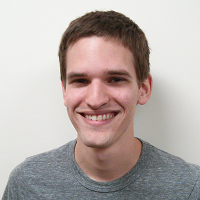
\includegraphics[width=0.3\linewidth]{Grant}
}

\textbf{Grant Hernandez} is a senior at the University of Central Florida. He will be
graduating with a Bachelor of Science in Computer Engineering this summer. In
his spare time, Grant writes lots of code, reverse engineers binaries, plays in cyber
Capture the Flag competitions, dabbles in computer graphics, and tinkers with
embedded systems. He will be attending the University of Florida in fall 2015
to begin his Ph.D in Computer Engineering with a security research lab.

\makebox[\textwidth][c]{
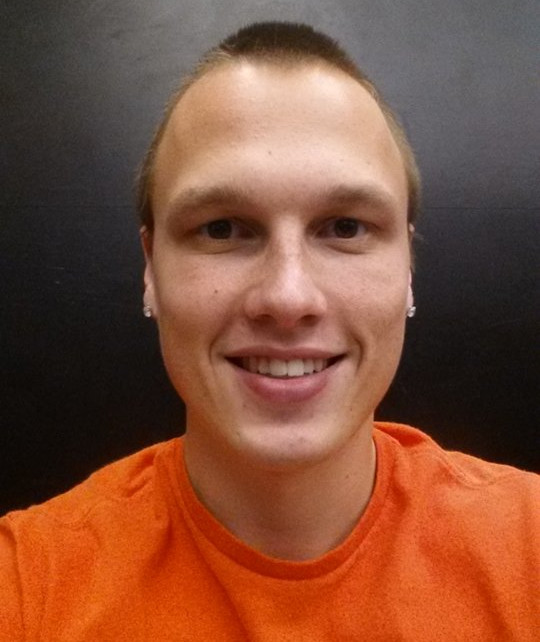
\includegraphics[width=0.3\linewidth]{Jimmy}
}

\textbf{Jimmy Campbell} is a senior at the University of Central Florida. He will be
receiving a Bachelor of Science in Computer Engineering in August 2015. His
interests include embedded programming, mobile development, and web back-end
development. Jimmy will be taking a full time position with Microsoft as a
Software Development Engineer after graduating.

\makebox[\textwidth][c]{
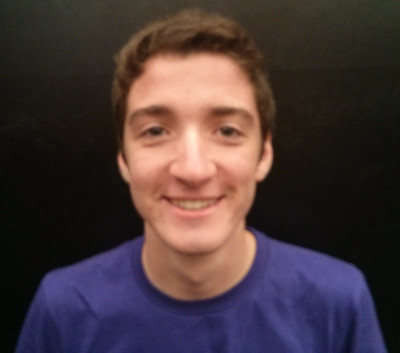
\includegraphics[width=0.3\linewidth]{Joseph}
}

\textbf{Joseph Love} is currently a senior at the University of Central Florida and will
receive his Bachelor of Science in Electrical Engineering in August of 2015. He
is currently working with Direct Beam Incorporated and plans to pursue his
masters in Electrical Engineering during the Fall of 2015 at UCF with a focus
in Electromagnetics.
